\chapter{{Manual Calculations}}
	
	{The proposed schematic configuration involves an input signal being fed into a common-emitter (CE) amplifier, which is then cascaded into another CE amplifier. This is followed by a common-collector (CC) amplifier that provides the output voltage with the desired level of amplification.}	
	
\begin{figure}[H]
    \centering
    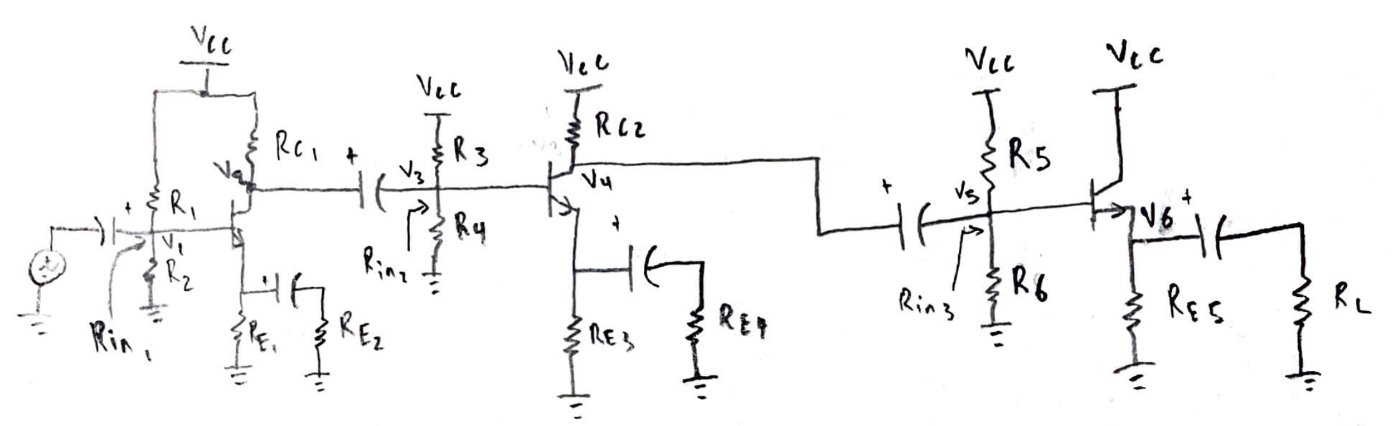
\includegraphics[width=16cm]{Pictures/Initial-Rough.png}
    \caption{{Initial Rough Sketch of the MultiStage Amplifier}}
    \label{initial-dia}
\end{figure}	
	
\section{Known Values}
\begin{itemize}
    \item \( V_{CC} = 10 \, \text{V} \)
    \item \( I_{DC} < 10 \, \text{mA} \)
    \item \( A_{vo} = 50 \)
    \item \( V_0 \geq 8 \, V_{pp} \)
    \item \( V_L \geq 4 \, V_{pp} \)
    \item \( R_{in} \geq 20 \, k\Omega \)
    \item All \( R \leq 220 \, k\Omega \)
\end{itemize}

\section{Common Collector (CC) Stage}
The gain for a CC stage is close to unity, so:
\[
A_{v3} = \frac{V_s}{V_l} \approx 1
\]

Since the total \( A_v \) (gain) at the end should be close to 50, we have:
\[
A_{vo} = A_{v1} \times A_{v2} \times A_{v3}
\]
\[
50 = A_{v1} \times A_{v2} \times 1
\]

For simplicity, \( A_{v1} \) and \( A_{v2} \) can have the same amplification:
\[
\sqrt{50} \approx 7.1
\]
\[
7.1 \times 7.1 = 50.41
\]
\[
A_{v1} = \frac{V_2}{V_1} = -7.1
\]
\[
A_{v2} = \frac{V_1}{V_3} = -7.1
\]

Both gains are \(-7.1\) because, overall, the circuit should become non-inverting at the end.

\section{Stages 1 and 2 (Common Emitter)}
Starting with stages 1 and 2:

Since \( A_{v1} = A_{v2} \), the collector current \( I_c \) for both CEs can be 400 \(\mu A\) as observed from the load line.

\[
g_m = \frac{I_c}{V_T} = \frac{400 \, \mu A}{26 \, mV} \approx 0.0154 \, S
\]

\[
I_B = 3.5 \, \mu A
\]

\[
\beta = \frac{400 \, \mu A}{3.5 \, \mu A} \approx 114.3
\]

\[
I_{B,DC} = 2 \, \mu A \, \text{(operating point/quiescent)}
\]

\section{Stage 3 (Common Collector)}
Assume \( R_{E3} = 1 \, k\Omega \) to be close to the \( R_L \) value.

\[
I_C = 10 \, mA \, \text{(from load line)}
\]

\[
\beta = \frac{I_C}{I_B} = \frac{10 \, mA}{65 \, \mu A} \approx 153.8
\]

\[
I_{B,DC} = 30 \, \mu A \, \text{(operating point/quiescent)}
\]

To ensure that the voltage at the base is not changed too much, the divider current should be much larger than \( I_B \). From the E24 series, a 91 \( k\Omega \) resistor can be used for \( R_5 \).

Also,
\[
g_m = \frac{10 \, mA}{26 \, mV} \approx 0.385 \, S
\]

\section{KCL at \(V_s\)}
\[
V_{CC} = 10V
\]

\begin{align*}
\text{KCL:} & \quad \frac{5 - 10}{91K} + \frac{5}{R_6} + 30 \, \mu A = 0 \\
            & \quad -24.945 \, \mu A + \frac{5}{R_6} = 0
\end{align*}

\[
R_6 = \frac{5 \, V}{24.945 \, \mu A} \approx 200.4 \, k\Omega
\]

\[
R_6 \approx 200 \, k\Omega
\]

\section{Assumptions}
5 V is approximated as the voltage where \(Q_{I, \text{operating point}}\) is from the graph.

Assume \(R_{E3} = 1 \, k\Omega\) due to the loading effect.

This process (going backwards) can continue to determine all the resistances.

\section{Stage 2 (CE)}
\begin{align*}
\text{KVL:} & \quad -4.25 + 0.7 + I_C \, (R_{E3}) = 0 \\
            & \quad -4.25 + 0.7 + (1 + \beta) \, I_B \, (R_{E3}) = 0
\end{align*}

\[
R_{E3} = \frac{3.5}{(1 + 114.3) \, (2 \, \mu A)} \approx 15.39 \, k\Omega
\]

\[
R_{E3} \approx 15 \, k\Omega
\]

\[
I_{C, DC} = \frac{V_{CC}}{R_C + R_{E3}} = \frac{10V}{400 \, \mu A} = 25 \, k\Omega
\]

\[
R_C + R_{E3} = 25 \, k\Omega \quad \Rightarrow \quad R_C = 25 \, k\Omega - 15 \, k\Omega = 10 \, k\Omega
\]

To find \(R_{E2}\), we need \(R_{in3}\):
\[
R_{in3} = R_5 // R_6 // \frac{\beta}{g_m + (\beta + 1)R_E}
\]

\[
R_{in3} = \frac{91K // 200K // \frac{153.8}{0.385} + (154.8)(1K)}{}
\approx 44.57 \, k\Omega
\]

\[
\frac{1}{10K} = \frac{1}{R_{E2}} + \frac{1}{44.57K} \quad \Rightarrow \quad R_{C2} \approx 13 \, k\Omega
\]

\textbf{(This is from Stage 3)}

Next, we can find \(R_E\) by using the gain equation. Note, since stage 1 and 2 are both CEs and have the same amplification, they will have the same biasing resistors, and the calculations will follow a similar procedure.

\section{Voltage Gain and Resistance Calculations}

\[
A_{v02} = \frac{V_z}{V_2} = -g_{m2} \left( \frac{R_{E2} // R_{in3}}{1 + g_{m2} R_E} \right)
\]

\[
-7.1 = -0.0154 \left(\frac{13K // 44.57K}{1 + 0.0154 \times R_{E}}\right)
\]

\[
-7.1 = \frac{-154.9924266 \times R_E}{1 + 0.0154 \times R_E}
\]

\[
R_E = \frac{-154.9924266 \times (-1)}{-7.1} \approx 1352.592159 \approx 1353 \, \Omega
\]

From this, the \(A_{v2}\) (with load) can be found:

\[
R_{in3} = \frac{91K // 200K // \frac{153.8}{0.385} + (154.8)(500)}{} \approx 34.67 \, k\Omega
\]

\[
A_{v2} \text{(with load)} = \frac{-0.0154 \times 13K}{34.67K} \times \frac{1}{1 + 0.0154 / 1353}
\]

\[
\approx -6.66 \approx -6.7
\]

\textbf{Note:} From stage 3, the resistance changed from 1k\(\Omega\) to 500\(\Omega\) when \(R_L\) is now used.

\section{Finding \(R_{E4}\) for Stage 2}

\[
R_E = 1353 \, \Omega \quad \Rightarrow \quad \frac{1}{1.3K} = \frac{1}{R_{E3} + R_{E4}} + \frac{1}{15K}
\]

\[
R_{E4} = 1423.357664 \, \Omega \approx 1.3K \, \Omega
\]

\textbf{Note:} Lowering emitter resistance yields more gain, so rounding down in intermediate calculations is acceptable to ensure the gain is met.

\section{Biasing Resistors}
Similar to stage 3, we need large enough resistors such that the divider current is much larger than \(I_B\). This is especially critical for CEs because if the divider current is too small, it can affect \(V_B\). Assume \(R_2 = 91K\) (from E24 series for simplicity's sake).

\section{Applying KCL at \(V_3\)}

\[
\frac{42.5 - 10}{91K} + \frac{4.25}{R_4} + 2 \, \mu A = 0
\]

\[
R_4 = \frac{4.25}{\frac{-2\mu A - \frac{42.5-10}{91K}}{}} \approx 68450.411092 \, \Omega
\]

\[
R_4 \approx 68K \, \Omega \quad \text{(round down since 70k not part of E24)}
\]

Next, 

\[
R_{in3} = R_3 // R_4 // \frac{\beta}{g_m + (\beta + 1)R_E}
\]

\[
R_{in3} = \frac{91K // 68K // \frac{114.3}{0.0154} + (115.3)(1353)}{} \approx 31432.72 \, \Omega \approx 31.433K \, \Omega
\]

\section{Stage 1 (Another CE)}

Lastly, we have stage 1, which is another common-emitter (CE) stage.

\[
I_{C,DC} = \frac{V_{CC}}{R_C + R_{E1}} = \frac{10V}{400 \, \mu A} = 25 \, k\Omega
\]

\[
25 \, k\Omega = R_C + R_{E1} \quad \therefore \quad R_C = 10 \, k\Omega
\]

\[
R_{C1} = \frac{R_C}{R_{C1} // R_{in2}} = 10 \, k\Omega = \frac{1}{\frac{1}{R_{C1}} + \frac{1}{31.433 \, k\Omega}}
\]

\[
R_{C1} = 14.66570242 \, k\Omega \approx 15 \, k\Omega
\]

\[
R_{E2} = R_E = \frac{R_{E1} // R_{E2}}{1.3 \, k\Omega} = \frac{1}{\frac{1}{R_{E2}} + \frac{1}{15 \, k\Omega}}
\]

\[
R_{E2} = 1423.357664 \, \Omega \approx 1.5 \, k\Omega \quad \text{(rounded to nearest E24 series)}
\]

We can use this and the same gain equation to find \( R_E \):

\[
A_{v1} = -g_m \left( \frac{R_C1}{R_{in2}} \right)
\]

\[
-7.1 = \frac{-0.0154 \times 14K // 31.433K}{1 + 0.0154 \times R_E}
\]

\[
R_E = \frac{-150.5202242 \times (-1)}{-7.1} \approx 1299.93 \, \Omega \approx 1.3 \, k\Omega
\]

Lastly, we can assume \( R_1 \) to be 91k\(\Omega\) (from the E24 series for simplicity's sake) so the divider current is significantly larger than the base current.

\section{Applying KCL, Solving for \(R_2\)}

\[
\frac{42.5 - 10}{91K} + \frac{4.25}{R} + 2 \, \mu A = 0
\]

\[
R_2 = \frac{4.25}{\frac{-2\mu A - \frac{42.5-10}{91K}}{}} \approx 61186.819 \times 10^{-5}
\]

\[
R_2 = 69450.41092 \, \Omega \quad R_2 \approx 68K \, \Omega \quad \text{(part of E24 series)}
\]

\section{Final Calculation for \(R_{in}\)}

\[
R_{in} = R_3 // 68K // \frac{\beta}{g_m + (\beta + 1)R_E}
\]

\[
R_{in} = \frac{91K // 68K // \frac{114.3}{0.0154} + (115.3)(1299)}{} \approx 31195.07046 \, \Omega \approx 31.195K \, \Omega
\]

\section{Capacitor Values and Quiescent Current Calculation}

Now that all the major calculations are done, capacitor values can be determined. Then the final quiescent current can be calculated as the final verification calculation for the circuit design, alongside the overall gain.

Values for \(C_1\) to \(C_6\): we can use the equation \(Z = \frac{1}{j\omega C}\).

It is important to note that emitter degeneration resistance is critical in order to maintain the gain of the CE stages. Larger capacitor values are expected for \(C_2\), \(C_4\), and \(C_6\). In contrast, \(R_{in1}\), \(R_{in2}\), \(R_{in3}\) values were relatively high already, so \(C_1\), \(C_3\), and \(C_5\) are not required to be as large (not as critical).

\section{Frequency Range and Impedance Calculations}

The frequency range is from 20 Hz to 50 kHz, so we can examine the impedance over this range. The sample values to test this are 100 \(\mu\)F and 10 \(\mu\)F.

\subsection{Worst Case}
\[
f = 20 \, \text{Hz}
\]
\[
C_2, C_4, C_6: \quad Z = \frac{1}{2\pi \times 20 \, \text{Hz} \times 100 \, \mu\text{F}} \approx 79.6 \, \Omega
\]
\[
C_1, C_3, C_5: \quad Z = \frac{1}{2\pi \times 20 \, \text{Hz} \times 10 \, \mu\text{F}} \approx 796 \, \Omega
\]

\subsection{Best Case}
\[
f = 50 \, \text{kHz}
\]
\[
C_2, C_4, C_6: \quad Z = \frac{1}{2\pi \times 50 \, \text{kHz} \times 100 \, \mu\text{F}} \approx 31.8 \, \text{m}\Omega
\]
\[
C_1, C_3, C_5: \quad Z = \frac{1}{2\pi \times 50 \, \text{kHz} \times 10 \, \mu\text{F}} \approx 0.32 \, \Omega
\]

\subsection{An Average Case (Using 1kHz as a Requirement from the Manual)}
\[
f = 1 \, \text{kHz}
\]
\[
C_2, C_4, C_6: \quad Z = \frac{1}{2\pi \times 1 \, \text{kHz} \times 100 \, \mu\text{F}} \approx 1.6 \, \Omega
\]
\[
C_1, C_3, C_5: \quad Z = \frac{1}{2\pi \times 1 \, \text{kHz} \times 10 \, \mu\text{F}} \approx 15.9 \, \Omega
\]

As seen by the calculated impedances, the selected capacitors of 100 \(\mu\)F and 10 \(\mu\)F should allow the circuit to maintain the gains.

\section{Final Gains}
\[
A_{vo} = -7.1 \times -7.1 = 50.41
\]
\[
A_v = -6.7 \times -7.1 = 47.57
\]

For \(A_{vo}\) and \(A_v\), we only multiply by 2 stages since stage 3 is a CC, so gain is approximately unity at stage 3. For \(A_v\) (with load), it is assumed the first CE stage will not feel the loading effect of \(R_L\), so we multiply the -6.7 by the initially assumed -7.1.

\section{Quiescent Current Calculation}
\[
I_{DC, \text{Total}} = I_{C1} + I_{R1} + I_{C2} + I_{R3} + I_{C3} + I_{R5}
\]

\[
= \beta I_{B1} + \frac{V_{CC}}{R_{F1} || R_{B2}} + \beta I_{B2} + \frac{V_{CC}}{R_{F3} || R_{B4}} + \frac{V_{CC}}{R_{F5} || R_{B6}}
\]

\[
= 114.3 \times (2 \, \mu A) + \frac{10}{91K // 68K} + 114.3 \times (30 \, \mu A) + \frac{10}{91K // 68K} + \frac{10}{200K // 91K}
\]

\[
\approx 0.00523 \, A \quad I_{DC, \text{Total}} = 5.23 \, mA \quad \text{(less than 10 mA, as required)}
\]

